\subsection{Intersection AIS and Satellite imagery}

Marine traffic detection using remote sensing approach is a commonly addressed task. \citeA{Brusch2011} showed how 
AIS and Synthetic Aperture Radar (SAR) data could be used in conjunction to detect vessels in small portions where
the satellite imagery tiles contain positional AIS messages. \citeA{Corbane2008} follow a similar approach joining
Vessel Monitoring System (VMS) and commercial satellite imagery to identify common features of shrimp boats. Although
these endeavors are working solutions, there is still wanting a strategy that can bring different sources of data that
can complement SAR data. One of these possible sources of data is high-resolution imagery, which until now has been 
restricted to commercial use only \cite{Greidanus2006}.

Our approach follows the work previously outlined since it is combining positional GPS data with remote sensing data. 
Nonetheless, it departs from it since it is mainly focused on UII activities, and also uses worldwide satellite imagery 
and AIS positional data. This work, at least in this preliminary stage, can work to create a comprehensive image 
database that can serve ultimately to validate the AIS data accuracy, and also the feasibility of joining different 
data sources to understand risky behaviors related to UII. 

The process of image retrieval was a tree step operation. First, we retrieve all the available images in \textit{Marine Areas} and
\textit{Ocean Areas} for our time frame (May 2016 to June 2017). The former are defined as areas is open waters; meanwhile the latter
are the areas near the continental land. This process yielded 187.038 images.\footnote{Additional 18.476 images were retrieved using 
Planet imagery only for the Torres Strait.}. Second, we overlap the bounding boxes of the imagery tiles with the AIS positional signals. 
This process was not only a spatial join, but also a time join which took into account the difference of time between the picture 
capture timestamp and the positional AIS timestamp. Figure \ref{overlap} shows the outcome of this step. In total, for Digital Globe,
the intersection retrieved 1.072 AIS positional signals (487 unique vessels). Third, we crop the images using a 800 meters square buffer 
of each the AIS coordinates inside the overlap. The Figure \ref{mosaic} shows the final outcome of this process.

\begin{figure}[H]
	\centering \caption{Overlap Digital Globe and AIS data (May 2016 - June 2017)}\label{overlap}
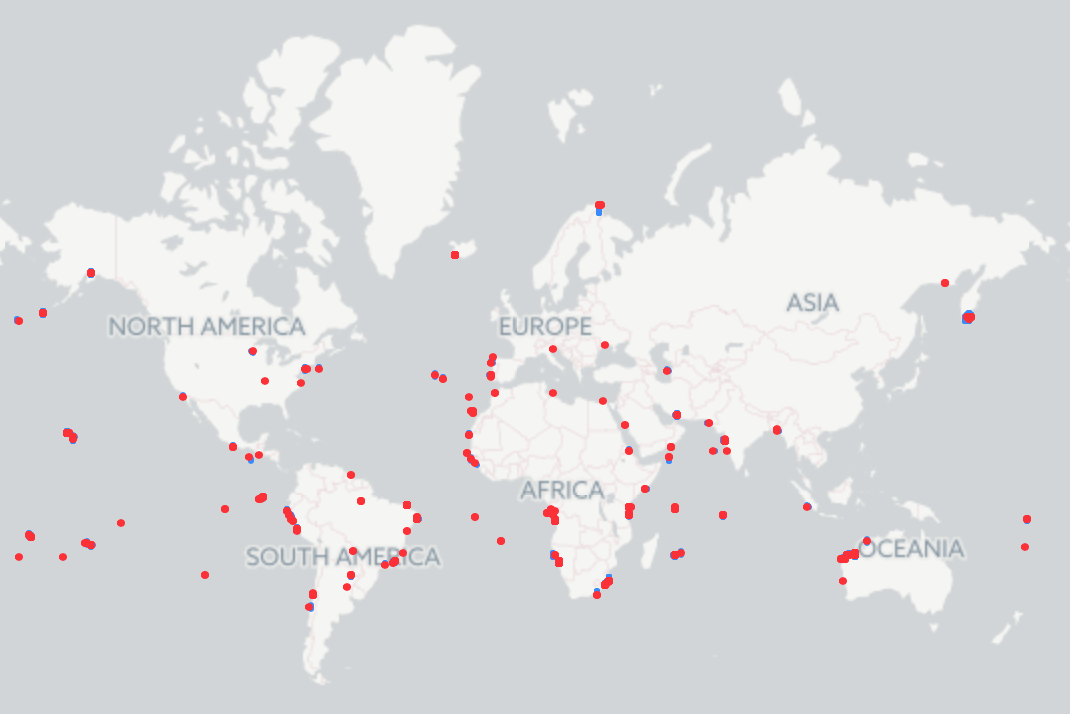
\includegraphics[width=0.6\linewidth]{images/overlap_gbdx.png} 
\begin{flushleft}
\rule{1.2in}{0em} \scriptsize Source: Digital Globe, Spire and OpenStreetMap. \\
\par
\end{flushleft}
\end{figure}

\begin{figure}[H]
	\centering \caption{Cropped images from Planet (May 2016 - June 2017)}\label{mosaic}
	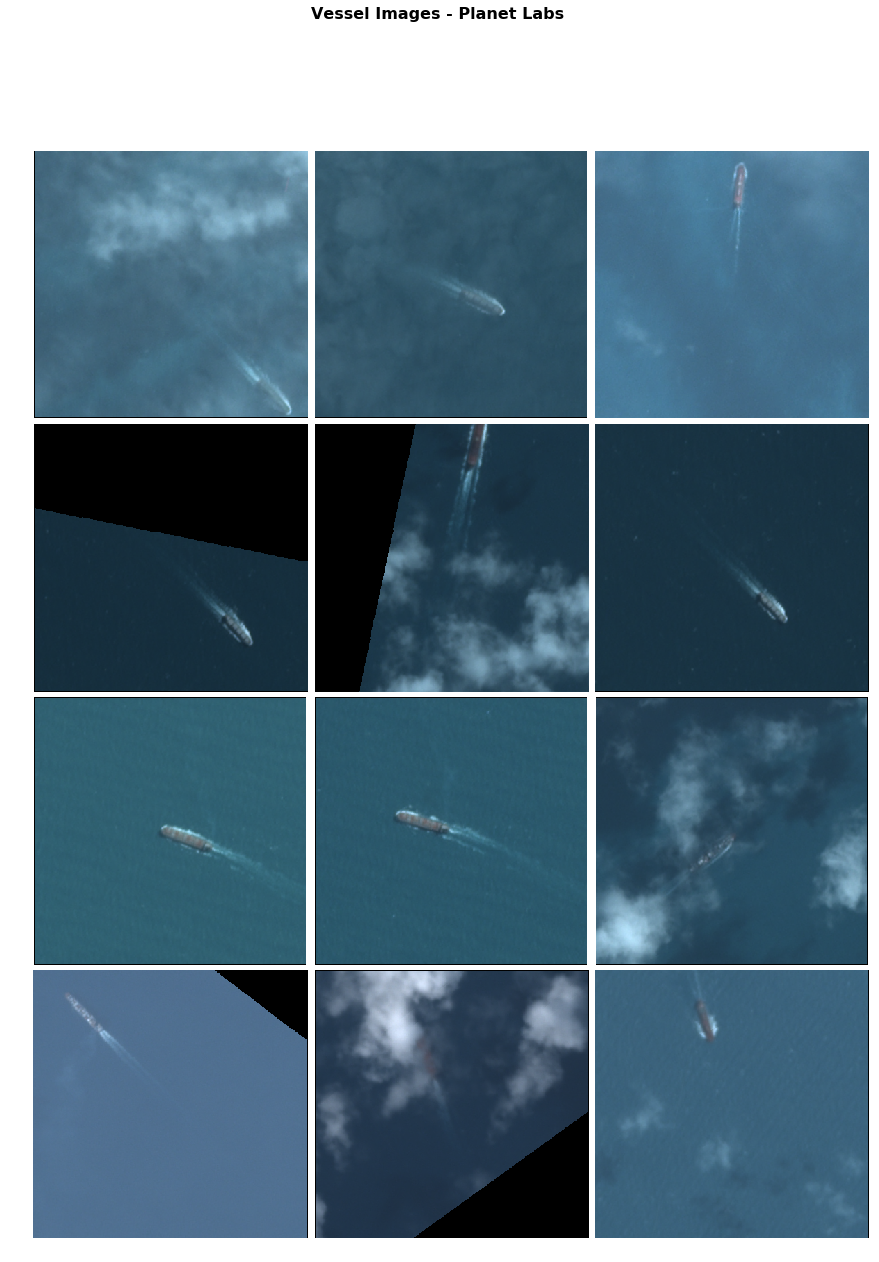
\includegraphics[trim={0 0 0 2cm},width=0.6\linewidth]{images/mosaic_planet_torres_strait.png} 
\begin{flushleft}
\rule{1.2in}{0em} \scriptsize Source: Planet and Spire. \\
\par
\end{flushleft}
\end{figure}


